\documentclass{yann}
\usepackage{tikz}

\newcommand{\Rpinf}{\Rp ∪\Acco{+∞}}
\newcommand{\sumni}{∑_{n=0}^{+∞}}
\newcommand{\Sanzn}{∑_n a_n z^n}
\newcommand{\Sanxn}{∑_n a_n x^n}
\newcommand{\Sbnzn}{∑_n b_n z^n}
\newcommand{\Scnzn}{∑_n c_n z^n}
\newcommand{\Ensembletq}[2]{\bigl\{#1\text{ tq }#2\bigr\}}
\newcommand{\me}{e} % {\mathrm{e}}
\newcommand{\I}{i} % {\mathrm{i}}

\begin{document}
\title{Séries entières}
\maketitle

% -----------------------------------------------------------------------------
\section{Rayon de convergence}

\Para{Définition}

On appelle \emph{série entière} toute série de fonctions de la forme $∑_n f_n$
où $(a_n)_{n∈ℂ}$ est une suite numérique et
où $\Fn{f_n}{ℂ}{ℂ}$ est définie par $f_n(z) = a_n z^n$.
La \emph{somme} de la série entière est la fonction \[ f \colon z \mapsto \sumni a_n z^n. \]

\Para{Lemme d'Abel}

Soit $\Sanzn$ une série entière et $z_0∈ℂ$ telle que la suite numérique $(a_n z_0^n)_{n∈ℕ}$ soit bornée.
Alors:
\begin{enumerate}
\item
  La série $\Sanzn$ converge absolument pour tout $z∈ℂ$ tel que $\Abs{z} < \Abs{z_0}$.
\item
  Plus précisément, la série de fonctions $\Sanzn$ converge normalement sur $\Ensembletq{z∈ℂ}{\Abs{z}≤r}$ dès que $0 ≤ r < \Abs{z_0}$.
\end{enumerate}

\Para{Attention!} Il n'y a pas toujours convergence normale (ni uniforme) sur $\Ensembletq{z∈ℂ}{\Abs{z}<\Abs{z_0}}$.

\Para{Définition}

Soit $\Sanzn$ une série entière.
Le \emph{rayon de convergence} $R∈\Rpinf$
de la série entière $\Sanzn$ est défini par
\begin{multline*}
  R = \sup \, \Bigl\{ \, r≥0 \text{ tel que} \\
  \text{la suite de terme général } \Abs{a_n} r^n \text{ est bornée} \, \Bigr\}.
\end{multline*}

\Para{Corollaire}

Soit $\Sanzn$ une série entière de rayon de convergence $R$ et $z_0 ∈ℂ$.
\begin{itemize}
\item
  Si $\Abs{z_0} < R$,
  la série numérique $∑_n a_n z_0^n$ converge absolument.
\item
  Si $\Abs{z_0} > R$,
  la série numérique $∑_n a_n z_0^n$ diverge grossièrement;
  plus précisément, la suite $(a_n z_0^n)_{n∈ℕ}$ n'est pas bornée.
\item
  Si $\Abs{z_0} = R$, la série peut ou non converger.
\end{itemize}

\Para{Définitions}

Soit $\Sanzn$ une série entière de rayon de convergence $R$.
\begin{itemize}
\item
  On appelle \emph{disque ouvert de convergence} de la série entière $\Sanzn$ l'ensemble
  \[ \Ensembletq{z∈ℂ}{\Abs{z}<R}. \]
\item
  On appelle \emph{cercle d'incertitude}
  (et parfois aussi, malheureusement, cercle de convergence)
  de la série entière $\Sanzn$ l'ensemble
  \[ \Ensembletq{z∈ℂ}{\Abs{z}=R}. \]
\end{itemize}

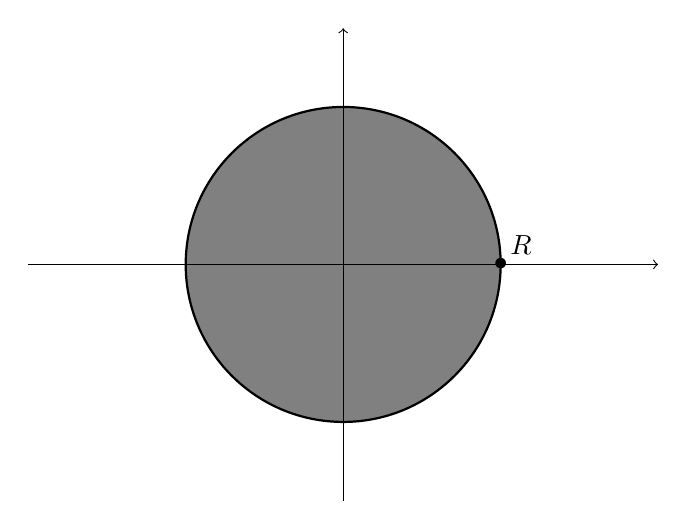
\begin{tikzpicture}[scale=2]
  \filldraw[thick,fill=gray] (0,0) circle (1) ;
  \draw[->] (-2,0) -- (2,0) ;
  \draw[->] (0,-1.5) -- (0,1.5) ;
  \draw (1,0) node {$\bullet$} node[above right] {$R$} ;
\end{tikzpicture}

% -----------------------------------------------------------------------------
\section{Détermination du rayon de convergence}

\subsection{Avec le lemme d'Abel}

\Para{Proposition}

Soit $\Sanzn$ une série entière de rayon de convergence $R$.
Soit $z_0∈ℂ$.
\begin{itemize}
\item
  Si $(a_n z_0^n)$ est bornée, alors $R≥\Abs{z_0}$.
\item
  Si $∑_n \Abs{a_n z_0^n}$ diverge, alors $R≤\Abs{z_0}$.
\end{itemize}

\subsection{Avec d'Alembert}

cf. exercice~\ref{exo:d'alembert}

\subsection{Avec les règles de comparaison}

\Para{Théorème}

Soit $\Sanzn$ et $\Sbnzn$ deux séries entières de rayons de convergence
respectivement $R_a$ et $R_b$.
\begin{enumerate}
\item
  S'il existe $α∈ℝ$ tel que $\Abs{a_n} = \GrandO \left( n^α\Abs{b_n} \right)$ quand $n\to+∞$, alors $R_a≥R_b$.
\item
  S'il existe $α∈ℝ$ et $K>0$ tel que $\Abs{a_n} \sim K n^α\Abs{b_n}$ quand $n\to+∞$, alors $R_a = R_b$.
\end{enumerate}

\pagebreak

% -----------------------------------------------------------------------------
\section{Opérations sur les séries entières}

\Para{Notations}
\begin{itemize}
\item
  Étant donné une série entière $\Sanzn$, on note $R_a$ son rayon de convergence et $f_a$ sa somme.
\item
  De même pour $\Sbnzn$ et $\Scnzn$.
\end{itemize}

\subsection{Somme}

\Para{Définition}

Soit $\Sanzn$ et $\Sbnzn$ deux séries entières.
On définit la \emph{somme} de ces deux séries entières
comme étant la série entière $\Scnzn$ où
\[ ∀n∈ℕ, \quad  c_n = a_n+b_n. \]

\Para{Proposition}

Dans ces conditions,
\begin{itemize}
\item
  $R_c≥\min(R_a,R_b)$ avec égalité si $R_a≠R_b$,
\item
  pour tout $z∈ℂ$ tel que $\Abs{z} < \min(R_a,R_b)$, on a $f_c(z) = f_a(z) + f_b(z)$.
\end{itemize}

\subsection{Multiplication par un scalaire}

\Para{Définition}

Soit $λ$ un scalaire et $\Sanzn$ une série entière.
On définit le \emph{produit} du scalaire et de la série entière
comme étant la série entière $\Sbnzn$ où
\[ ∀n∈ℕ, \quad  b_n =λa_n. \]

\Para{Proposition}

Dans ces conditions,
\begin{itemize}
\item
  $R_b = R_a$ si $λ≠0$, et $R_b = +∞$ si $λ= 0$,
\item
  pour tout $z∈ℂ$ tel que $\Abs{z} < R_a$, on a $f_b(z) =λf_a(z)$.
\end{itemize}

\subsection{Produit de Cauchy}

\Para{Définition}

Soit $\Sanzn$ et $\Sbnzn$ deux séries entières.
On définit le \emph{produit de Cauchy} de ces deux séries entières
comme étant la série entière $\Scnzn$ où
\[ ∀n∈ℕ, \quad c_n = ∑_{k=0}^n a_k b_{n-k}. \]

\Para{Proposition}

Dans ces conditions,
\begin{itemize}
\item
  $R_c ≥\min(R_a,R_b)$,
\item
  pour tout $z∈ℂ$ tel que $\Abs{z} < \min(R_a,R_b)$, on a $f_c(z) = f_a(z) f_b(z)$.
\end{itemize}

% -----------------------------------------------------------------------------
\section{Propriétés de la somme}

\Para{Théorème}[continuité sur le disque ouvert de convergence]

Soit $\Sanzn$ une série entière de rayon de convergence $R$ et de somme $f$.
Alors $f$ est continue sur le disque ouvert de convergence
\[ \Ensembletq{z∈ℂ}{\Abs{z}<R}. \]

\Para{Proposition}

Soit $\Sanzn$ une série entière de rayon de convergence $R$.
Alors les deux séries entières suivantes:
\begin{itemize}
\item
  la \og{}dérivée formelle\fg{} $∑_n b_n z^n$ où $b_n = (n+1)a_{n+1}$,
\item
  la \og{}primitive formelle\fg{} $∑_n c_n z^n$ où $c_n = \frac{a_{n-1}}{n}$
\end{itemize}
ont également un rayon de convergence égal à $R$.

\Para{Théorème}[primitivation terme à terme]

Soit $\Sanxn$ une série entière de rayon de convergence $R$ et de somme $f$.
Une primitive de $f$ sur $\intO{-R,R}$ est donnée par
\[ F \colon x \mapsto \sumni a_n \frac{x^{n+1}}{n+1} = ∑_{n=1}^{+∞} \frac{a_{n-1}}{n} x^n. \]

\Para{Proposition}[dérivation terme à terme]

Soit $\Sanxn$ une série entière de rayon de convergence $R$ et de somme $f$.
Alors $f$ est une fonction de classe $\CC1$ sur $\intO{-R,R}$
et $∀x∈\intO{-R,R}$,
\[ f'(x) = ∑_{n=1}^{+∞} n a_n x^{n-1} = \sumni (n+1) a_{n+1} \, x^n. \]

\Para{Théorème}[généralisation]

Soit $\Sanxn$ une série entière de rayon de convergence $R$ et de somme $f$.
Alors $f$ est une fonction de classe $\CC∞$ sur $\intO{-R,R}$
et $∀p∈ℕ$, $∀x∈\intO{-R,R}$,
\[ \begin{aligned} f^{(p)}(x)
    &= ∑_{n=p}^{+∞} a_n n(n-1) \cdots (n-p+1) x^{n-p} \\
    &= \sumni a_{n+p} \frac{(n+p)!}{n!} x^n.
\end{aligned} \]

\Para{Corollaire}

Soit $\Sanxn$ une série entière de rayon de convergence $R>0$ et de somme $f$.
Alors pour tout $n∈ℕ$, on a
\[ a_n = \frac{f^{(n)}(0)}{n!}. \]

% -----------------------------------------------------------------------------
\section{Fonctions développables en séries entières}

\Para{Notation}
\begin{itemize}
\item
  $I$ désigne un intervalle de $ℝ$ tel qu'il existe
  $ε> 0$ tel que $\intO{-ε,ε}⊂I$.
\end{itemize}

\Para{Définition}

Soit $\Fn fIℂ$.
On dit que $f$ est \emph{développable en série entière} au voisinage de $0$
si et seulement si il existe $α> 0$
et une série entière $\Sanxn$ de rayon de convergence $R≥α$ tels que
$\intO{-α,α}⊂I$ et
\[ ∀x∈\intO{-α,α} \+ f(x) = \sumni a_n x^n. \]

\Para{Proposition}

Si $\Fn fIℂ$ est développable en série entière au voisinage de $0$,
alors il existe $α> 0$ tel que
$f$ soit de classe $\CC∞$ sur $\intO{-α,α}$.

\Para{Définition}

Soit $\Fn fIℂ$ une fonction de classe $\CC∞$.
On appelle \emph{série de Taylor} de $f$ au voisinage de $0$
la série entière
\[ ∑_n a_n z^n \quad \text{où} \quad∀n∈ℕ\+ a_n = \frac{f^{(n)}(0)}{n!}. \]

\Para{Théorème}[unicité du développement en série entière]

Soit $\Fn fIℂ$ développable en série entière au voisinage de $0$.
Alors tout développement en série entière de $f$ au voisinage de $0$
est égal à sa série de Taylor au voisinage de $0$.

\Para{Corollaire}

Soit $\Fn fIℂ$ développable en série entière au voisinage de $0$.
Alors $f$ admet un développement limité au voisinage de $0$ à tout ordre,
et ce développement limité s'obtient en tronquant le développement en série entière.

\Para{Proposition}

Soit $\Fn fIℂ$.
Alors $f$ est développable en série entière au voisinage de $0$
si et seulement si il existe $α> 0$ tel que
\begin{itemize}
\item
  $f$ est de classe $\CC∞$ sur $\intO{-α,α}$,
\item
  la série de Taylor de $f$ converge sur $\intO{-α,α}$,
\item
  $f$ soit égale à la somme de se série de Taylor sur $\intO{-α,α}$.
\end{itemize}

% -----------------------------------------------------------------------------
\section{Fonctions usuelles}

\subsection{Exponentielle complexe}

\Para{Proposition}

La série entière $∑_n \frac{z^n}{n!}$ a un rayon de convergence infini.
Notons $φ\colon z \mapsto \sumni \frac{z^n}{n!}$ sa somme.
On montre successivement:
\begin{enumerate}
\item
  $∀(z_1,z_2)∈ℂ^2$, $φ(z_1+z_2) =φ(z_1)φ(z_2)$
\item
  $∀x∈ℝ$, $φ(x) = \me^x$
\item
  $∀θ∈ℝ$, $φ(\Iθ) = \cosθ+ \I \sinθ$
\item
  $∀(x,y)∈ℝ^2$, $φ(x+\I y) = \me^x(\cos y + \I \sin y)$
\end{enumerate}

\Para{Définition}

On appelle \emph{exponentielle} la fonction définie par
\[ ∀z∈ℂ, \quad \exp(z) = \sumni \frac{z^n}{n!}. \]
Il s'agit d'une série entière de rayon de convergence infini.
On note fréquemment $\me^z$ au lieu de $\exp(z)$.

\Para{Proposition}

Soit $z∈ℂ$ fixé et $\Fonction{φ}{ℝ}{ℂ}{t}{\exp(tz)}$\\
Alors $φ$ est de classe $\CC∞$ et
\[ ∀n∈ℕ \+ ∀t∈ℝ, \quad φ^{(n)}(t) = z^n \exp(tz). \]

\subsection{Trigonométrie}

\Para{Définitions}

On définit, pour tout $z∈ℂ$:
\begin{multicols}{2}
  \begin{itemize}
  \item
    $\cos z = \frac{\me^{\I z} + \me^{-\I z}}{2}$
  \item
    $\sin z = \frac{\me^{\I z} - \me^{-\I z}}{2\I}$
  \item
    $\ch z = \frac{\me^{z} + \me^{-z}}{2}$
  \item
    $\sh z = \frac{\me^{z} - \me^{-z}}{2}$
  \end{itemize}
\end{multicols}
Il s'agit de prolongement des fonctions cosinus, sinus, cosinus hyperbolique
et sinus hyperbolique, classiquement définies sur $ℝ$.

\Para{Proposition}

\begin{itemize}
\item
  Les formules usuelles de trigonométries restent valables,
  notamment $∀(a,b)∈ℂ^2$:
  \begin{itemize}
  \item
    $\cos(a+b) = \cos(a) \cos(b) - \sin(a) \sin(b)$
  \item
    $\sin(a+b) = \sin(a) \cos(b) + \cos(a) \sin(b)$
  \end{itemize}
\item
  On peut passer de la trigonométrie directe
  à la trigonométrie hyperbolique sachant que $∀z∈ℂ$:
  \begin{multicols}{2}
    \begin{itemize}
    \item
      $\ch(\I z) = \cos(z)$
    \item
      $\sh(\I z) = \I\sin(z)$
    \item
      $\cos(\I z) = \ch(z)$
    \item
      $\sin(\I z) = \I\sh(z)$
    \end{itemize}
  \end{multicols}
\end{itemize}

\Para{Proposition}

On a, pour tout $z∈ℂ$:
\begin{itemize}
\item
  $\DS \cos z  = ∑_{n=0}^{+∞} \frac{(-1)^n}{(2n)!} \, z^{2n}$
\item
  $\DS \sin z  = ∑_{n=0}^{+∞} \frac{(-1)^n}{(2n+1)!} \, z^{2n+1}$
\item
  $\DS \ch z = ∑_{n=0}^{+∞} \frac{1}{(2n)!} \, z^{2n}$
\item
  $\DS \sh z = ∑_{n=0}^{+∞} \frac{1}{(2n+1)!} \, z^{2n+1}$
\end{itemize}

Il s'agit de séries entières de rayon de convergence infini.

\subsection{$x \mapsto (1+x)^α$}

\Para{Proposition}

Soit $α∈ℝ$ et $\Fn{f}{\intO{-1,+∞}}{ℝ}$ définie par $f(x)=(1+x)^α$.
Alors $f$ est développable en série entière au voisinage de $0$.
Plus précisément, on a
\[ ∀x∈\intO{-1,1}, \quad (1+x)^α= ∑_{n=0}^{+∞} a_n x^n \]
où $a_0 = 1$ et \[ ∀n∈\Ns \+ a_n = \frac{1}{n!}∏_{k=0}^{n-1} (α-k). \]
On note parfois $a_n = \binom{α}{n}$.
Il s'agit d'une série entière de rayon de convergence égal à~1
si $α∉ℕ$, et $+∞$ si $α∈ℕ$.

\Para{Remarque}

Si $α∈ℤ$, le développement est également valable dans $ℂ$
\[ ∀z∈ℂ\text{ tel que } \Abs{z}<1, \quad
(1+z)^α=∑_{n=0}^{+∞} a_n z^n, \]
où $(a_n)_{n∈ℕ}$ est défini comme ci-dessus.

\Para{Exemple}

Déterminer le développement en série entière de la fonction $x\mapsto\arcsin x$.

\subsection{Fractions rationnelles}

\Para{Méthode}

Pour obtenir un développement en série entière (au voisinage de $0$)
d'une fraction rationnelle, on peut:
\begin{itemize}
\item
  la décomposer en éléments simples $\frac{1}{(x-a)^n}$ où $a∈ℂ^*$;
\item
  remarquer que $\frac{1}{(x-a)^n} = (-a)^{-n} \left[ 1+\left(-\frac xa\right) \right]^{-n}$;
\item
  se ramener à $(1+u)^α$.
\end{itemize}

On obtient une série entière de rayon de convergence~$\Abs{a}$.

% -----------------------------------------------------------------------------
\section{Exercices}

\Exercice[règle de d'Alembert pour les séries entières]\label{exo:d'alembert}

Soit $\Sanzn$ une série entière et $R$ son rayon de convergence.
On suppose que:
\begin{itemize}
\item
  il existe $N∈ℕ$ tel que pour tout $n≥N$ on ait $a_n≠0$,
\item
  $\left|\frac{a_{n+1}}{a_n}\right| \Toninfℓ∈\Rpinf$.
\end{itemize}

On cherche à montrer que $R = \frac1ℓ$
où, par convention, $\frac{1}{0}=+∞$ et $\frac{1}{+∞}=0$.

\begin{enumerate}
\item
  On suppose $ℓ∈\Rps$ et $z∈\Cs$.
  \begin{enumerate}
  \item
    Montrer que la série $∑_n a_n z^n$ converge si $ℓ\abs{z} < 1$
    et diverge si $ℓ\abs{z} > 1$.
  \item
    En déduire $R = \frac1{ℓ}$.
  \end{enumerate}
\item
  Traiter les cas $ℓ=0$ et $ℓ=+∞$.
\end{enumerate}

\Exercice

Déterminer le rayon de convergence de la série entière $∑_n a_n z^n$ pour:
\begin{multicols}{2}
  \begin{enumerate}
  \item
    $a_n = n!$
  \item
    $a_n = \ln n$
  \item
    $a_n = \binom{3n}{n}$
  \item
    $a_n = n^{√n}$
  \item
    $a_n = \frac{n^n}{n!}$
  \item
    $a_n$ vaut la somme des diviseurs de $n$
  \item
    $a_n = \cos n$.
    On pourra commencer par montrer que $(\cos n)_{n∈ℕ}$ ne converge pas vers $0$.
  \item
    $a_n = \frac{\sin n}{n}$
  \item
    $\arctan\left(\frac1{n^α}\right)$
  \item
    $a_n = \frac{α^n}{n} + \frac{β^n}{n^2}$
  \item
    $a_n = \tan\left(\frac{nπ}{7}\right)$
  \item
    $a_{2n} = 0$,  $a_{2n+1} = \frac{(-1)^n}{\ch n}$
  \item
    $a_{3n} = \frac{1}{n^2+1}$, $a_{3n+1}=\frac{1}{n!}$ et $a_{3n+2} = α^n$
  \item
    $a_0 > 0$, \\ $a_{n+1} = \ln(1+a_n)$
  \item
    $a_n = \lfloor \me^n \rfloor$
  \item
    $a_n = \frac{1}{n!} \left( 1+\frac1n \right)^{n^2}$
  \item
    $a_n$ est la $n$-ième décimale de $e$
  \end{enumerate}
\end{multicols}

\Exercice

Déterminer le rayon de convergence et la somme des séries entières suivantes:
\begin{multicols}{2}
  \begin{enumerate}
  \item
    $∑_{n≥0} n^{(-1)^n} x^n$
  \item
    $∑_{n≥0} n^2 x^n$
  \item
    $∑_{n≥0} \left( \frac n3 - \left\lfloor \frac n3 \right\rfloor \right) x^n$
  \item
    $∑_{n≥0} \frac{n^2+4n-1}{n!} \, x^n$
  \item
    $∑_{n≥1} \left( ∑_{k=1}^n \frac1k \right) x^n$
  \item
    $∑_{n≥1} \frac{x^n}{1+2+\cdots+n}$
  \item
    $∑_{n≥0} \sin(nθ) \, x^n$
  \item
    $∑_{n≥1} \frac{\sin(nθ)}{n} \, x^n$
  \item
    $∑_{n≥0} \frac{\cos(nθ)}{n!} \, x^n$
  \item
    $∑_{n≥0} \left( ∑_{k=0}^n \frac{1}{k!} \right) x^n$
  \item
    $∑_{n≥0} a_n x^n$ où $(a_n)_{n∈ℕ}$ vérifie la récurrence $a_{n+3}=a_{n+2}+a_{n+1}-a_n$.
  \end{enumerate}
\end{multicols}

\Exercice

Développer en série entière, au voisinage de~$0$, les fonctions de $x$ suivantes:
\begin{multicols}{2}
  \begin{enumerate}
  \item
    $\frac{\ln(1+x)}{1+x^2}$
  \item
    $\ln(x^2-5x+6)$
  \item
    $\me^{-x} \sin x$
  \item
    $\frac{1-x\chα}{1-2x\chα+x^2}$
  \item
    $\arctan\left( \frac{1}{√3} + x \right)$
  \item
    $\arcsin x$
  \item
    $\frac{\me^x}{1-x}$
  \item
    $\me^{x^2} ∫_0^x \me^{t^2} \D t$
  \end{enumerate}
\end{multicols}

\Exercice

On suppose que les séries entières $∑_n α_n z^n$ et $∑_n β_n z^n$ ont même rayon $R$ de convergence
et que pour tout $n∈ℕ$, on ait $\Abs{α_n} ≤ \Abs{a_n} ≤ \Abs{β_n}$.
Quel est alors le rayon de convergence de $∑_n a_n z^n$?

\Exercice

Soit $\Sanzn$ une série entière de rayon de convergence~$R>0$.
Quel est le rayon des séries entières suivantes:
\begin{multicols}{2}
  \begin{enumerate}
  \item
    $∑_n \frac{a_n}{n!} z^n$
  \item
    $∑_n n^α a_n z^n$
  \item
    $∑_n a_n z^{7n+3}$
  \item
    $∑_n a_n^α z^n$ où $α∈ℝ$
  \item
    $∑_n \frac{a_n}{n^{42}+\cos n+1} \, z^n$
  \item
    $∑_n S_n z^n$ \\ où $S_n = ∑_{k=0}^n a_k$
  \end{enumerate}
\end{multicols}

\Exercice

\begin{enumerate}
\item
  Soit $(u_n)$ une suite réelle telle que
  $∀n≥n_0$, $u_{n+p}≤αu_n$.
  Montrer qu'il existe une constante $K$ telle que pour tout $n∈ℕ$ on ait l'inégalité
  $u_n≤Kα^{n/p}$.
\item
  Soit $p∈\Ns$ et $(a_n)_{n∈ℕ}$ une suite de complexes non nuls vérifiant
  $\lim_\ninf \left| \frac{a_{n+p}}{a_n} \right| = ℓ$.
  Déterminer le rayon de convergence de la série entière $∑_n a_n z^n$.
\end{enumerate}

\Exercice[théorème de continuité au bord]\label{exo:continuite_bord}

Soit $\Sanxn$ une série entière de rayon de convergence $R$ et $f$ sa somme.
\begin{enumerate}
\item
  On suppose que $∑_n \Abs{a_n} R^n$ converge.
  Montrer que $f$ est continue sur le disque fermé de convergence $[-R,R]$.
\item
  \emph{Lemme}: Soit $∑_n b_n$ une série numérique convergente;
  on ne la suppose pas nécessairement absolument convergente.

  \begin{enumerate}
  \item
    On pose $g_n(x) = b_n x^n$.
    Montrer que la série de fonctions $∑_n g_n$ converge uniformément sur $[0,1]$.
  \item
    En déduire que la fonction $g(x) = ∑_{n≥0} b_n x^n$ est continue sur $[0,1]$.
  \end{enumerate}
\item
  \emph{Application:}

  \begin{enumerate}
  \item
    On suppose que $∑_n a_n R^n$ converge.
    Montrer que $f$ est continue sur $[0,R]$.
  \item
    On suppose que $∑_n a_n (-R)^n$ converge.
    Montrer que $f$ est continue sur $[-R,0]$.
  \end{enumerate}
\end{enumerate}

\Exercice
\begin{enumerate}
\item
  Soit $f \colon x \mapsto \arctan x$.
  \begin{enumerate}
  \item
    Développer $f$ en série entière au voisinage de 0.
  \item
    A priori, sur quel intervalle a-t-on l'égalité entre $f$ et son développement en série entière?
  \item
    En utilisant le théorème de continuité au bord (exercice~\ref{exo:continuite_bord}),
    montrer que ce développement est encore valable pour $x=1$.
  \item
    En déduire la valeur de $\DS ∑_{n=0}^{+∞} \frac{(-1)^n}{2n+1}$.
  \end{enumerate}
\item
  Avec la même méthode, calculer
  \[ ∑_{n=1}^{+∞} \frac{1}{n(2n+1)} \quad\text{et}\quad
  ∑_{n=1}^{+∞} \frac{(-1)^n}{n(2n+1)}. \]
\end{enumerate}

\Exercice

Soit $f$ l'unique fonction $ℝ\toℝ$ solution de
\[ \begin{cases} y' - 2xy = 1 \\ y(0) = 0 \end{cases} \]
\begin{enumerate}
\item
  Calculer le développement en série entière de $f$ de deux façons différentes:

  \begin{enumerate}
  \item
    en résolvant l'équation différentielle, puis en développant la solution en série entière,
  \item
    en supposant $f$ développable en série entière et en injectant ce développement dans l'équation différentielle pour obtenir une récurrence
  \end{enumerate}
\item
  En déduire une expression simple de la somme
  \[ ∑_{k=0}^n \frac{(-1)^k}{2k+1} \binom{n}{k}. \]
\end{enumerate}

\Exercice

Pour $x$ réel, on pose $\DS f(x) = ∑_{n=1}^{+∞} \frac{x^n}{√{n}}$.
\begin{enumerate}
\item
  Déterminer le rayon de convergence $R$ de la série entière définissant $f$.
\item
  Étudier la convergence de la série entière en~$1$ et en~$-1$.
\item
  Établir la continuité de $f$ en~$-1$.
\item
  Déterminer la limite de $f$ en~$1$.
\end{enumerate}

\Exercice

Soit $f(z) = ∑_{n=0}^{+∞} a_n z^n$ la somme d'une série entière de rayon de convergence infini.
\begin{enumerate}
\item
  Calculer $\DS I_n = \frac{1}{2π}∫_0^{2π} f(r\me^{\Iθ}) \me^{-n\Iθ} \Dθ$.
\item
  Soit $\DS M(r) = \sup_{\Abs{z}=r} \Abs{f(z)}$. Montrer que $\Abs{a_nr^n}≤M(r)$.
\item
  En déduire que, si $f$ est bornée sur $ℂ$, alors $f$ est constante;
  il s'agit de la version faible du théorème de Liouville.
\end{enumerate}

\Exercice

Soit $(u_n)_{n∈ℕ}$ la suite définie par
$u_0=1$ et $∀n∈ℕ$, \[ u_{n+1} = ∑_{k=0}^n u_k u_{n-k} \]
Soit $f(x) = ∑_{n=0}^{+∞} u_n x^n$.
On note $R$ le rayon de convergence de cette série entière.
\begin{enumerate}
\item
  On suppose que $R > 0$.
  \begin{enumerate}
  \item
    Montrer que $∀x∈\intO{-R,R} ∖ \acco{0}$, $f^2(x) = \frac{f(x)-1}{x}$.
  \item
    En déduire une expression de $f$. \emph{Attention, c'est un peu subtil à cause du signe.}
  \end{enumerate}
\item
  Soit $\DS g(x) = \frac{1-√{1-4x}}{2x}$.
  \begin{enumerate}
  \item
    Développer $g$ en série entière. Quel est son rayon $R'$ de convergence?
  \item
    Montrer que $xg^2(x) = g(x) - 1$ pour tout $x∈\intO{-R,R}$.
  \item
    En déduire que le développement en série entière de $g$ est $∑_{n≥0} u_n x^n$.
  \end{enumerate}
\item
  Donner une expression simple de $u_n$.
\end{enumerate}

\emph{Remarque}: les $(u_n)$ s'appellent les \emph{nombres de Catalan}.
Ils possèdent de nombreuses interprétations combinatoires.

\Exercice

Pour $x∈ℝ$, on pose $\DS f(x) = ∑_{n=0}^{+∞} \frac{\cos(2^n x)}{n!}$.
\begin{enumerate}
\item
  Montrer que $f$ est définie et de classe $\CC∞$ sur $ℝ$.
\item
  Observer que le rayon de convergence de sa série de Taylor en~$0$ est nul.
\end{enumerate}

\end{document}

% ------------------------------------------------------------------------------
% ------------------------------------------------------------------------------
% ------------------------------------------------------------------------------

\Exercice
\begin{enumerate}
\item
  Montrer que les deux intégrales
  $∫_0^1 \frac{\ln t}{1-t} \D t$ et
  $∫_0^1 \frac{\ln t}{1-t^2} \D t$ convergent.
\item
  En développant en série entière $\frac{1}{1-t}$ et $\frac{1}{1-t^2}$, calculer leurs valeurs.
\item
  En déduire $∫_0^{+∞} \frac{t\D t}{\sh t}$.
\end{enumerate}
